\chapter{システム構成と3Dモデルの取得}

本章では，本論文で扱う三つの料理マニピュレーション研究に共通する基盤として，ロボットシステムの構成と，対象物および作業環境の3Dモデル取得方法を述べる．
本論文の中心的な立場は，3Dモデルを単なる形状の記録として扱うのではなく，動作生成，力学解析，および制御設計のための計算基盤として利用する点にある．
このため，各タスクに固有の詳細なアルゴリズムを述べる前に，それらの前提となる共通の計測・モデリング過程を明確にしておく必要がある．

本論文で扱うタスクは，液体を注ぐ操作，食材表面に沿った皮むき操作，および切断時における食材の安定把持である．
これらは対象物の物理特性や要求される制御方式こそ異なるものの，いずれも対象物の三次元形状や作業空間の幾何情報を把握し，そこから操作に必要な量を導出するという点で共通している．
具体的には，注ぐ操作では容器内部形状から容積や液面検出に必要な情報を得る必要があり，皮むき操作では食材表面形状から工具軌道を生成する必要があり，切断時把持では食材形状上で接触点候補を生成し，把持安定性を評価する必要がある．

このような観点から，本章ではまず各研究で用いたロボットシステムを整理し，次にRGB-Dカメラを用いた多視点計測による3Dモデル生成手順を述べる．
さらに，生成した3Dモデルから抽出される幾何情報と，各タスクにおけるその利用方法をまとめる．
最後に，3Dモデル取得の精度評価について述べ，本章で構築する基盤の妥当性を示す．



\section{ロボットシステムの構成}

本論文で扱う注ぐ動作，皮むき動作，および把持の研究では，共通の双腕ロボットシステムを用いた．
本節では，まず三つの研究に共通するロボット，視覚センサ，および力覚センサについて述べ，その後，各研究におけるエンドエフェクタ設計を説明する．

\subsection{ロボット}

実験には，三菱電機製の7自由度マニピュレータ PA10-7C を2台用いた．
両アームは卓上作業に適するよう床面から700\,mmの高さに設置し，ベース座標系間の距離は$Y$軸方向に804\,mmとした．
各アームのベース座標系は，ロボット前方を$x$軸，ロボットから見て左方向を$y$軸，鉛直上方を$z$軸とするように設定した．
また，双腕協調作業を統一的に記述するため，左アームのベース座標系原点を世界座標系の原点として用いた．
\begin{figure}[ht]
    \centering
    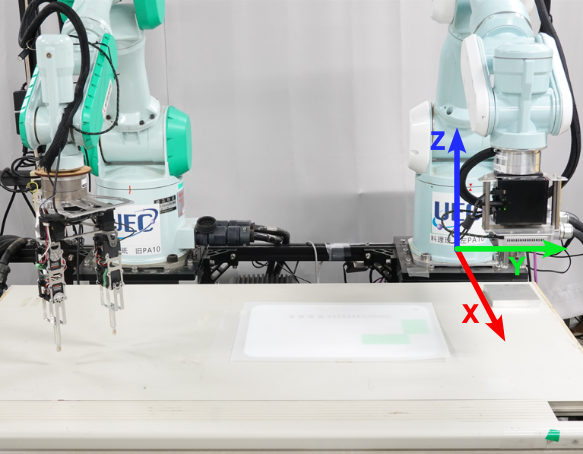
\includegraphics[width=.8\linewidth]{fig//chp3/ICRA_RobotEnv.png}
    \caption{ロボットシステムと座標系}
    \label{fig:robot_env}
\end{figure}

本研究では，ロボット手先にツールを装着した状態で各種作業を実行するため，手先座標系に加えてツール座標系を定義した．
ツール座標系の位置は装着した道具の中心に設定し，姿勢は各ツールの幾何学的関係に応じて与えた．
これにより，ロボット手先そのものではなく，実際に対象へ作用する道具先端の位置姿勢を基準として動作を記述・制御できる．
この構成は，三つの研究に共通するハードウェア基盤である．

\subsection{視覚センサ}

対象物および作業環境の3D情報取得には，Intel RealSense D435 を用いた．
本センサはRGB画像と深度画像を同時に取得できるRGB-Dカメラであり，容器，食材，液面近傍，および反射を含む表面に対しても比較的安定した深度情報を取得できる．
図\label{fig:robot_camera}のように，カメラは主としてグリッパ前面に取り付け，ロボットアームの動作により視点を能動的に変化させることで，複数視点から点群を取得した．
\begin{figure}[ht]
    \centering
    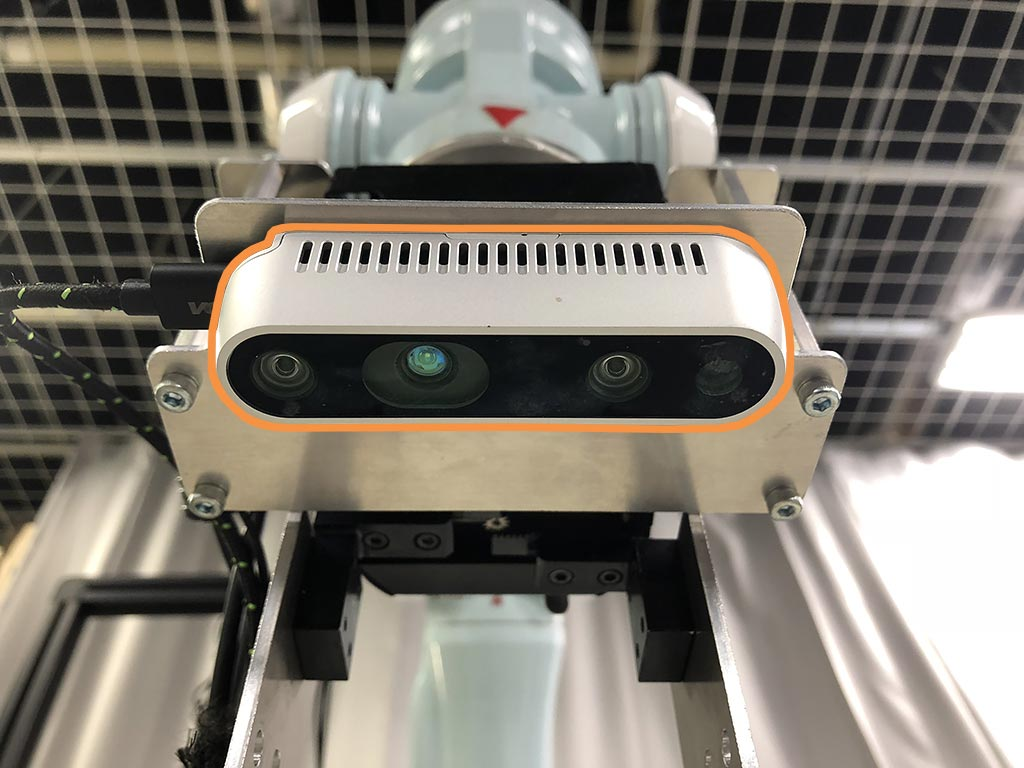
\includegraphics[width=.7\linewidth]{fig//chp3/Realsense.jpg}
    \caption{手首に取り付けたIntel RealSense D435}
    \label{fig:robot_camera}
\end{figure}

取得した点群は，各時刻におけるロボット姿勢とカメラの取り付け関係に基づいて世界座標系へ変換し，統合した3Dモデルとして利用する．
この3Dモデルは，注ぐ動作では容器内部形状の推定と容積計算に，皮むき動作では食材表面形状の把握と工具軌道生成に，切断時把持では接触候補点の生成と把持安定性評価に用いられる．

\subsection{力覚センサ}

ロボットと対象物との接触を伴う操作を安定に実現するため，両腕の手首部には Leptrino 製の6軸力覚センサ PFS080YA501U6S を装備した．
このセンサはUSB経由で制御用PCに接続し，作業中に発生する力およびモーメントを計測する．
データシート（図\ref{fig:force_sensor_spec}）に基づけば，定格荷重500\,N，分解能$1/4000$より，力の分解能は約0.125\,Nである．
\begin{figure}[ht]
    \centering
    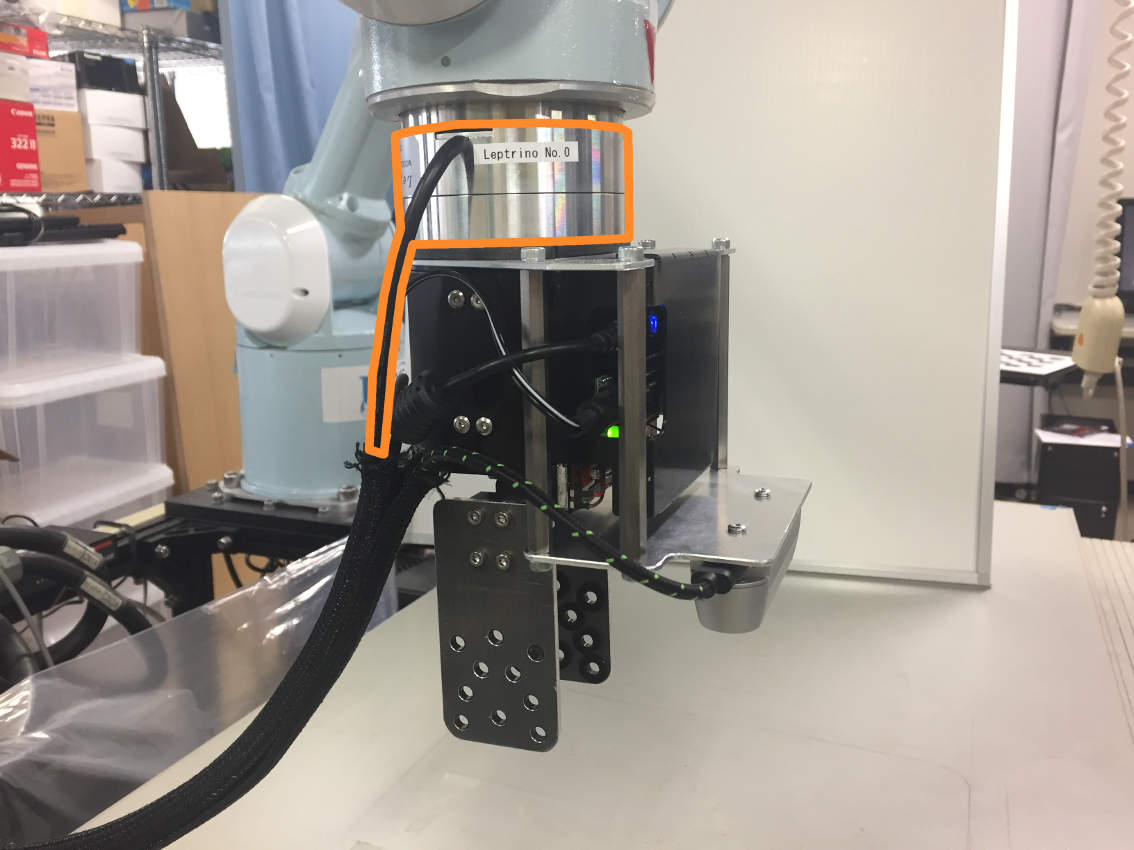
\includegraphics[width=.7\linewidth]{fig/chp3/ForceSensor.jpg}
    \caption{手首に取り付けたLeptrino製の6軸力覚センサー}
    \label{fig:force_sensor_install}
\end{figure}
\begin{figure}[ht]
    \centering
    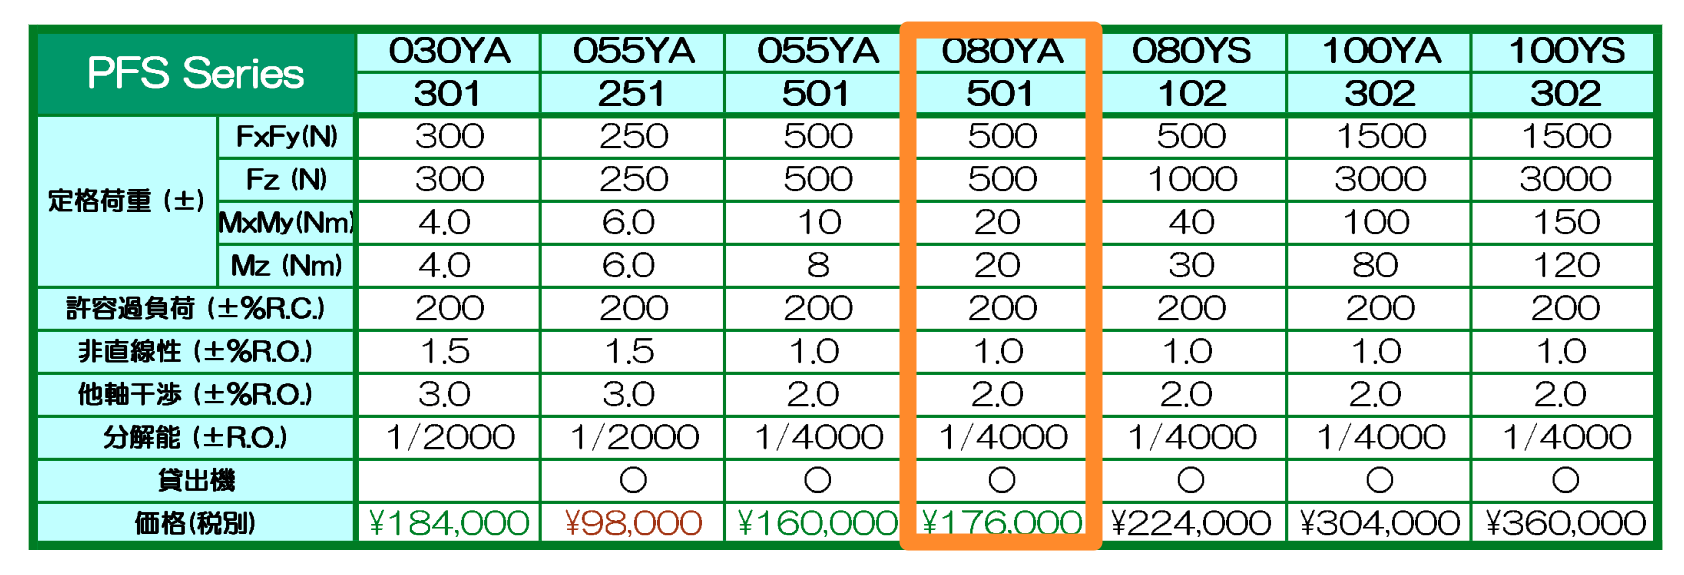
\includegraphics[width=1\linewidth]{fig//chp3/ForceSensor-performence.png}
    \caption{PFS080YA501U6Sの仕様書}
    \label{fig:force_sensor_spec}
\end{figure}

力覚情報は，特に工具と対象表面との接触が重要となる皮むき動作において有効であり，接触状態の監視および制御入力の設計に用いた．
また，本論文では，3Dモデルに基づく幾何学的解析に加えて，接触に伴う力学的情報も操作設計の一部として扱うため，力覚センサはそのための共通計測基盤として位置づけられる．

\subsection{注ぐ動作におけるエンドエフェクタ設計}

注ぐ動作では，各種容器を安定に把持し，必要に応じて持ち上げ，傾ける必要がある．
そこで，平行グリッパを基盤とし，その指先アルミ板に容器把持用のエンドエフェクタを取り付けた．
本研究では，対象容器の形状差に対応するため，2種類のエンドエフェクタを用いた．

第1のエンドエフェクタ（図\ref{fig:pour_endeffactor_1}）は，ボウルやカップのように開口縁を有する容器を対象としたものである．
平行グリッパの開口幅のみでは把持が困難な場合を想定し，容器本体ではなく縁部を把持できるように設計した．
また，把持時の摩擦力を高めるため，接触面には小型のスポンジを取り付けた．
\begin{figure}[ht]
    \centering
    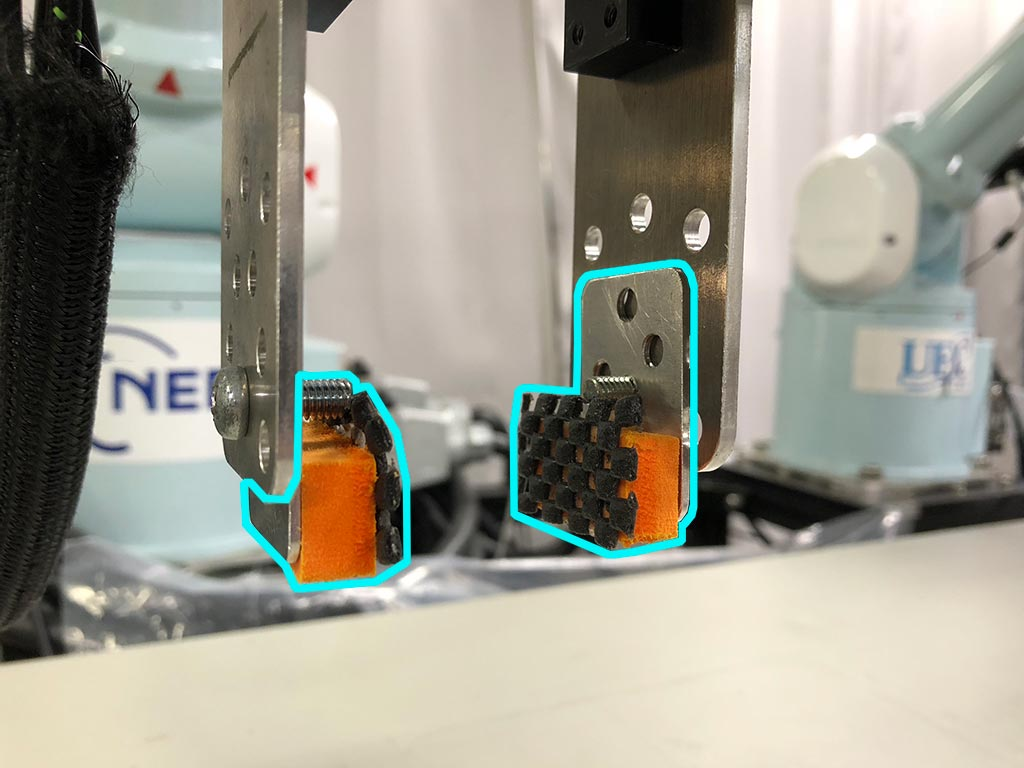
\includegraphics[width=.7\linewidth]{fig/chp3/PourEndFactor-1.jpg}
    \caption{注ぐ動作のエンドエフェクタ1の様子}
    \label{fig:pour_endeffactor_1}
\end{figure}

第2のエンドエフェクタ（図\ref{fig:pour_endeffactor_2}）は，外形寸法が比較的小さく，グリッパ開口幅内に収まる容器を確実に把持することを目的としたものである．
こちらも把持安定性向上のため，接触面に薄いスポンジを取り付けた．
このように，注ぐ動作におけるエンドエフェクタ設計では，容器形状の多様性に対して，把持様式を切り替えられることを重視した．
\begin{figure}[ht]
    \centering
    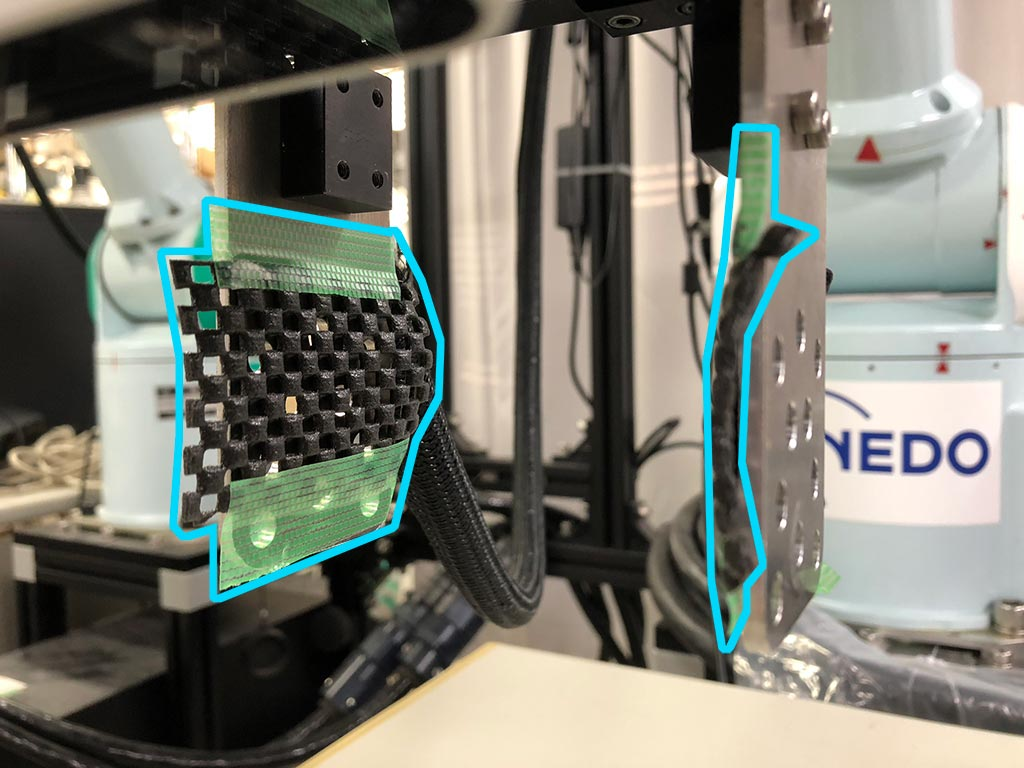
\includegraphics[width=.7\linewidth]{fig/chp3/PourEndFactor-2.jpg}
    \caption{注ぐ動作のエンドエフェクタ2の様子}
    \label{fig:pour_endeffactor_2}
\end{figure}

\subsection{皮むき動作におけるエンドエフェクタ設計}

皮むき動作では，一方の腕でピーラーを操作し，他方の腕で食材を安定に支持する必要がある．
このため，両腕とも平行グリッパを基盤としつつ，役割に応じて異なるエンドエフェクタを装着した．

工具側のエンドエフェクタ（図\ref{fig:pour_endeffactor_2}）としては，ピーラーをロボット手先へ固定するためのアダプタを設計した．
このアダプタにより，ピーラーの刃先位置と姿勢をツール座標系として明確に定義でき，食材表面形状に基づいて生成した軌道に従って刃先を安定に移動させることが可能となる．
\begin{figure}[ht]
    \centering
    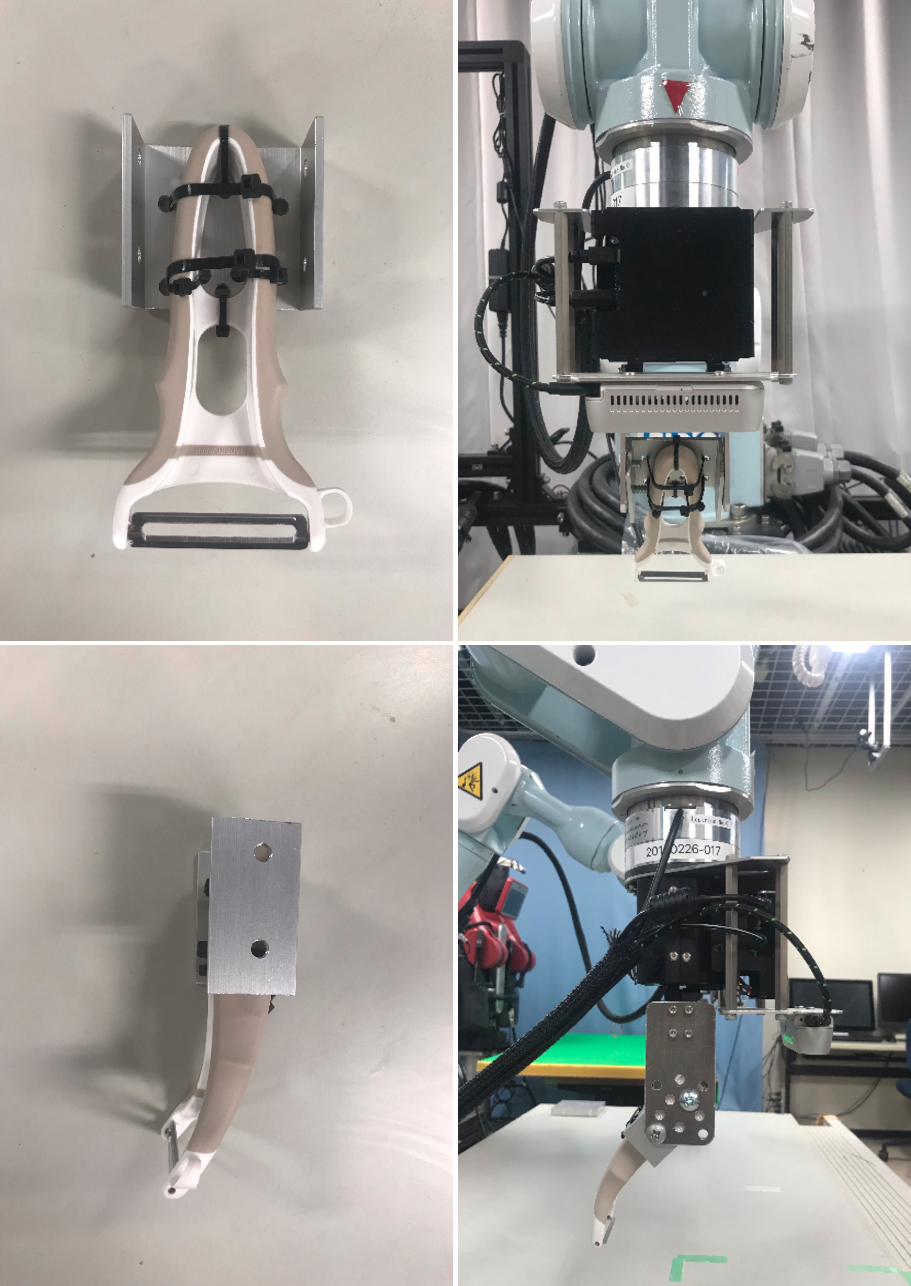
\includegraphics[width=.7\linewidth]{fig/chp3/PeelingEndeffector-2.pdf}
    \caption{皮むき動作のピーラー側エンドエフェクタの様子}
    \label{fig:peeling_endeffactor_2}
\end{figure}

食材固定側のエンドエフェクタとしては，食材に刺した串を安定に固定するための専用機構を用いた．
細長い串は通常の平行グリッパでは毎回同じ位置に保持することが難しいため，$V$字溝を有する把持部を設け，串が一定位置に自然に収まるように設計した．
これにより，食材の姿勢再現性が向上し，皮むき軌道の安定な実行が可能となる．
\begin{figure}[ht]
    \centering
    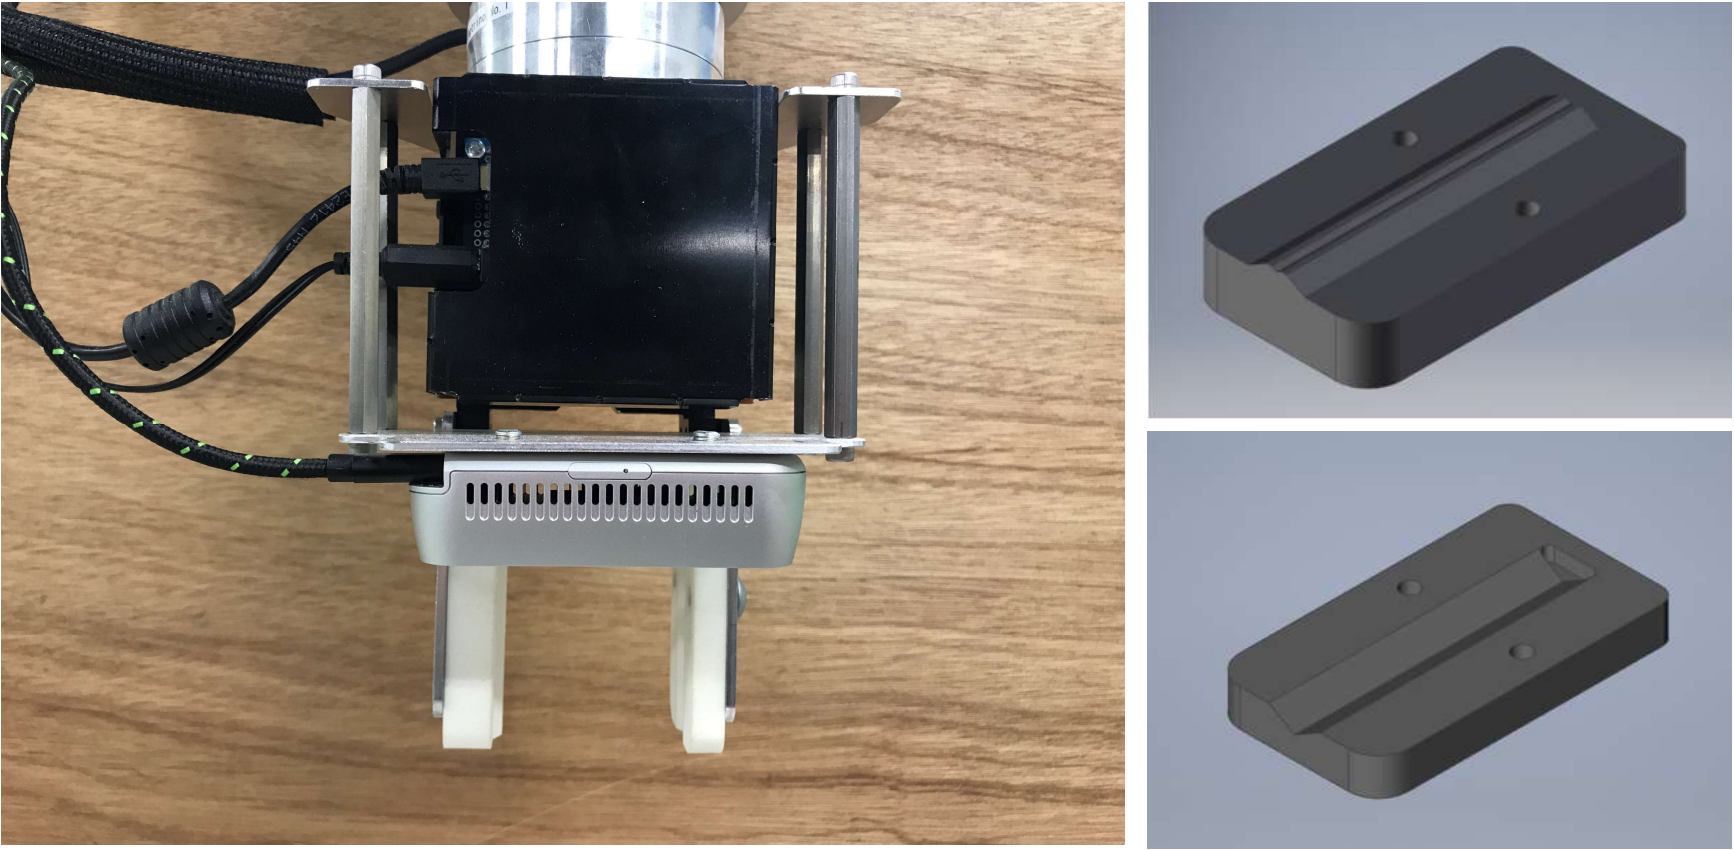
\includegraphics[width=.5\linewidth]{fig/chp3/PeelingEndeffector-1.png}
    \caption{皮むき動作の食材固定側エンドエフェクタの様子}
    \label{fig:peeling_endeffactor_1}
\end{figure}


\subsection{安定把持におけるエンドエフェクタ設計}

安定把持の研究では，左腕に食材把持用の指型ハンドを，右腕に包丁固定用の高把持力平行グリッパを装着した．
右腕側の平行グリッパは，包丁をロボットへ剛に固定することを目的としており，切断時に発生する外力を安定に伝達できるようにした．
一方，左腕側では，食材形状に応じて接触点を柔軟に選択できることが重要であるため，多関節の指型ハンドを用いた．

食材把持用ハンドとしては，3軸2指のサーボハンドを用いた．
各指には FUTABA RS405CB を使用し，最大トルクは48.0\,$\mathrm{kgf \cdot cm}$，角度分解能は0.1\,degである．
各指の関節構成は $z$-$y$-$y$-tip とし，指先位置を制御するために，ヤコビアンに基づく指関節のみの逆運動学を用いた．
この構成により，食材表面上に生成した候補接触点へ指先を誘導し，把持安定性の評価に基づいて適切な接触配置を実現できる．

\begin{figure}[ht]
    \centering
    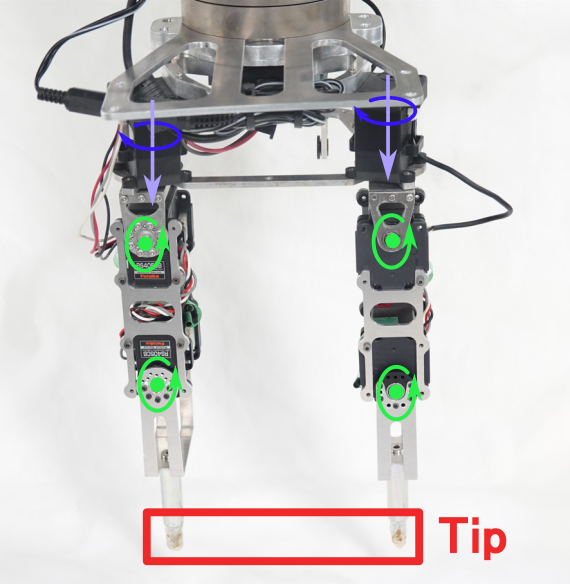
\includegraphics[width=.5\linewidth]{fig/chp3/ICRA_RobotHand.png}
    \caption{把持に使用する指ハンド}
    \label{fig:robot_hand}
\end{figure}

このように，切断時把持におけるエンドエフェクタ設計では，包丁側には高剛性な固定機構を，食材側には形状適応性を有する多指ハンドを割り当てることで，切断時の外力と把持安定性の両立を図った．



\section{3Dモデル取得のためのセンシング手順}

\subsection{多視点観測の基本方針}

RGB-Dカメラによって得られる点群は単一視点の観測結果であるため，遮蔽，反射，および視野制約の影響を受けやすい．
特に，容器内部のような深い凹形状，食材の裏面，あるいは作業台に接している領域は，単一視点では十分に観測できない場合が多い．
そこで本研究では，ロボットアームを用いてカメラ姿勢を能動的に変化させ，複数視点から対象物を観測することで，より完全な3Dモデルを構築した．

多視点観測では，対象物の周囲を囲むように複数の視点を設定し，各視点においてカメラ座標系で点群を取得する．
その後，各点群を世界座標系へ変換し，単一の点群として統合する．
この操作により，単視点では欠落していた部分を相補的に補完できる．

\subsection{タスクごとの観測手順}

注ぐ動作では，注ぐ側容器および目標容器の内部形状が重要であるため，容器開口部から内部を観測できる視点を含めて複数姿勢から点群を取得した．
特に，容器の底部や側壁の形状は容積推定に直接影響するため，できる限り死角を減らすように観測姿勢を設計した．

皮むき動作では，食材表面に沿った工具軌道を生成するため，主として食材外表面の観測が重要となる．
このため，食材の回転軸や作業時の姿勢を考慮しつつ，表面形状を十分に捉えられる複数視点からRGB点群を取得した．
また，皮むきの進行に応じて色分布が変化するため，必要に応じてRGB情報も併用した．

切断時把持では，接触点候補の探索や包丁運動との干渉判定のために，食材全体の形状を可能な限り完全に取得する必要がある．
そのため，対象周囲からの観測に加え，必要に応じて対象物を持ち上げ，底面の点群も取得した．
これにより，食材全体の外形をより正確に再構成し，把持候補点の生成精度を高めた．

\section{点群統合と3Dモデルの生成}

\subsection{座標変換と点群統合}

各視点で取得された点群は，まずカメラ座標系から世界座標系へ変換される．
この変換には，ロボットの関節角から得られる順運動学と，カメラとエンドエフェクタ間の相対姿勢を与えるキャリブレーション結果を用いる．
得られた各視点の点群を同一座標系へ写像することで，対象物に対する統合点群を構成する．

点群統合の際には，視点ごとの計測誤差やノイズの影響を低減するために，外れ値除去およびダウンサンプリングを行う．
これにより，不要なノイズ点の影響を抑えつつ，後続の幾何処理や探索計算に適した密度の点群へ整形することができる．

\subsection{前処理と平滑化}

統合された点群に対しては，必要に応じてテーブル平面の除去，クラスタリング，対象物クラスタの選択，および平滑化を行う．
例えば，容器モデルの生成では，まずテーブル面を除去し，残った点群をクラスタリングして対象容器に対応するクラスタを抽出する．
皮むきおよび切断時把持では，対象食材に対応する点群を選択し，移動最小二乗法などを用いて表面形状を平滑化する．

平滑化は，表面法線の計算や断面輪郭の抽出を安定化するために重要である．
生の点群には深度センサ特有のばらつきが含まれるため，そのままでは局所法線や曲率の推定が不安定になることがある．
適度な平滑化により，形状の大局的特徴を保ちながら，後続処理に適したモデルを得ることができる．

\subsection{不足領域の補完}

3Dモデル生成において特に問題となるのは，遮蔽や設置面の影響により，対象物の一部が観測できないことである．
容器では深い底部が欠損しやすく，食材では接地面や把持に隠れた部分が欠損しやすい．
この問題に対し，本研究では単なる単視点観測に依存せず，多視点化や対象物の持ち上げを用いて不足領域を補完した．

ただし，観測を追加しても完全な復元が困難な場合は残る．
このような場合でも，本論文では後続タスクに必要な情報がどの程度取得できているかを重視する．
すなわち，常に完全な幾何モデルを要求するのではなく，容積推定，軌道生成，把持点候補生成などの各タスクで必要十分な精度を満たすことを目標とした．

\section{3Dモデルから抽出される情報と各タスクでの利用}

本論文において3Dモデルは，単なる点の集合ではなく，各種の幾何情報を抽出するための基盤として利用される．
まず，容器モデルに対しては，z軸方向に一定間隔でスライスを行い，各断面の面積を求めることで容積分布を推定できる．
この情報は，目標量を注ぐための液量推定や，角度と注出量の関係計算に利用される．
また，容器の軸平行境界ボックスを計算することで，液面検出の対象領域を限定することもできる．

次に，食材表面モデルに対しては，表面法線，断面輪郭線，および局所的な形状変化を抽出できる．
皮むき動作では，食材の回転軸を含む平面で点群をスライスし，そこから断面輪郭線を取り出すことで，ピーラーの刃先が倣うべき基準軌道を生成する．
さらに，表面法線の変化を用いて軌道を複数の直線セグメントへ簡略化し，実機で実行しやすい形式へ変換する．

切断時把持では，3Dモデル上の表面点がそのまま接触候補点の探索空間となる．
各候補点集合に対し，包丁から加わる力や摩擦力とのつり合いを評価し，把持に必要な指先力の大きさ，方向，および分散を評価する．
すなわち，3Dモデルは接触候補を生成するだけでなく，それらを力学的に評価するための幾何基盤としても機能する．

以上のように，本論文における3Dモデルの役割は，認識結果の保存ではなく，幾何解析から制御設計へ接続するための計算代理として位置づけられる．
同じRGB-D点群モデルであっても，注ぐ，皮むき，切断時把持という異なるタスクにおいて，抽出される情報とその使われ方が異なる点に，本論文のアプローチの特徴がある．

\section{3Dモデル取得精度の評価}

3Dモデルを基盤として操作設計を行う以上，その取得精度を評価しておくことは重要である．
本論文では，三つの研究で使用されるモデル取得方法の妥当性を評価するために，既知形状を有する対象を用いて点群合成精度を調べる．
具体的には，CADで対象物を設計し，3Dプリンタにより実体を作製した上で，RGB-Dカメラによって観測・再構成したモデルと比較する方法が考えられる．

評価指標としては，第一に「設計」「実際」「認識」に基づく体積比較が挙げられる．
これにより，単に表面形状が見た目に近いかどうかではなく，容器容積や物体体積といったタスク上重要な量がどの程度再現されているかを確認できる．
第二に，設計モデルと認識モデルの位置合わせを行い，その残差誤差を求めることで，形状一致度を評価できる．
第三に，対象形状の種類ごとに誤差傾向を比較することで，深い容器，半切り食材，曲率の大きい対象などに対する本手法の得意・不得意を把握できる．

本論文では，モデル取得誤差が各タスクに及ぼす影響も併せて検討する．
例えば，注ぐ動作では容器底部の欠損が容積推定誤差につながりやすい．
皮むき動作では表面法線推定の乱れが軌道生成精度に影響する．
切断時把持では接触点位置のずれが力学評価の誤差につながる．
したがって，単に点群再構成精度を数値で示すだけでなく，その誤差が後続処理にどう伝播するかという観点から評価することが望ましい．

\section{本章のまとめ}

本章では，本論文の三つの研究に共通する基盤として，ロボットシステムの構成と3Dモデル取得方法を述べた．
まず，研究ごとに用いたハードウェア構成は完全には同一でないものの，双腕ロボット，末端近傍のRGB-Dカメラ，および世界座標系への点群統合という基本思想が共通していることを示した．
次に，多視点観測による点群取得，座標変換に基づく統合，前処理と平滑化，不足領域の補完を通して，対象物および作業環境の3Dモデルを構築する手順を述べた．
さらに，そのモデルから抽出される幾何情報が，容積推定，軌道生成，把持候補探索といった各タスクの中核処理に利用されることを示した．

以上より，本章で構築した3Dモデル取得と利用の基盤は，後続章で述べる各タスク固有の方法の前提となる．
第4章では未知容器への定量注ぎ，第5章では曲面食材の皮むき，第6章では切断時の安定把持について，それぞれ本章で述べた基盤の上に具体的な解析・動作生成・制御方法を示す．

